%!TEX root = ../../thesis.tex
%!TEX enableSynctex = true
%*******************************************************************************
%*********************************** First Chapter *****************************
%*******************************************************************************

\ifpdf
    \graphicspath{{Chapters/intro/Figs/Raster/}{Chapters/intro/Figs/PDF/}{Chapters/intro/Figs/}}
\else
    \graphicspath{{Chapters/intro/Figs/Vector/}{Chapters/intro/Figs/}}
\fi

\chapter{Introduction}

% \noindent Fluorescence microscopy has experienced a scientific renaissance over the last 20 years through advances in new fluorescent proteins and super-resolution optical microscopy, both of which were awarded with Nobel Prizes in Chemistry.
Fluorescence microscopy is one of the cornerstones of modern biology, but has generally been limited to 2D culture dishes.
Light-sheet microscopy, a recent advance which was awarded Nature Method of the Year 2014, allows fast, non-invasive 3D imaging across an entire organism.
This works by decoupling illumination and detection such that the microscope only illuminates a thin section of tissue at a time.
By scanning this `light-sheet' through an organism we can image in 3D more quickly and with less damage than other techniques such as confocal microscopy.
%we can construct a detailed 3D image with sub-cellular resolution.

%Traditional techniques are slow.
% Super-resolution microscopy allows an improvement in optical imaging resolution previously thought to be physically impossible.
% Super res great, but only good in 2D. %Confocal is 3D but is slow and "force entire" and isn't super res.
% lightsheet is fast, 3D and can be supe res, by seperating objective
%We can now visually inspect live biological specimens in real time and at protein length scales.
%These imaging techniques do however require long acquisition and exposure times, and so force the entire biological sample to be flooded with light, which subjects delicate samples to harmful radiation.
%Light sheet Fluorescence Microscopy is distinct from these techniques in that it introduces an additional excitation lens at right angles to the detection, confining the illumination to the plane of interest and minimising harm to the sample.
%This decoupling then allows for fast, non-invasive 3D imaging across an entire organism.
%This decoupling then allows for fast, deep and non-invasive volumetric imaging.
%Light sheet Fluorescence Microscopy was Nature Method of the Year 2014 and promises to be the future standard, disrupting 400 years of established microscopy.
%These advances have been so revolutionary that Light-sheet fluorescence microscopy was awarded Nature Method of the Year 2014.

During the first year of my PhD I designed and built a custom light-sheet microscope which we have applied to studying the cell mechanics of developing embryos.
%Cell mechanics plays a vital role in the development of organisms;
Internal stresses within tissues induce cellular migrations that can govern the organism's resultant anatomy.
We have developed a technique to mechanically probe deep tissue using magnetism.
By embedding a magnetic bead in an embryo we can use a controllable, non-invasive magnetic field to move the bead.
By pushing a magnetic bead and allowing it to relax we can fit a model to its trajectory and so extract local mechanical properties.
% Comparing results between embryos that are genetically modified to no longer produce different key proteins provides an understanding of their roles in embryonic development. %TODO Reword
The mechanical roles of key proteins in embryonic development can be inferred by comparing results between genetically modified embryos.
%Using light-sheet imaging we can rapidly visualise entire live cells, permitting an unprecedented opportunity to observe and induce cell migration and tissue formation.
%Our investigations so far have demonstrated that rho-kinase, in embryonic development increases cell stiffness
%is inaccurate. %and %TODO add something.+
Our investigations so far have contradicted previous reports that rho-kinase increases cell stiffness in embryonic development. These results are currently being prepared for publication with our collaborators.

% Looking ahead, I intend to  single magnetic bead tracking to that of single virus particle tracking, going from the microscopic to the nanoscopic.
Looking ahead, I intend to move from tracking single magnetic beads to tracking single virus particles, going from the microscopic to nanoscopic scale.
Virus particles (virions) invade host cells and hijack their machinery to replicate and then spread. %their disease
By visualising the journey of virions through the cell we may reveal weaknesses in infection pathways.
%Light-sheet microscopy is the only technique capable of volumetrically tracking virions, which are both exceptionally small and fast.
Light-sheet microscopy is better suited than other techniques for tracking virus trafficking in 3D as virions are exceptionally small and fast.
We intend to study Herpes Simplex Virus~1 which causes cold sores and genital herpes.
Furthermore, it serves as a biological model for other Herpesviruses which are associated with many serious diseases including chickenpox and certain lymphomas.
%and life-threatening conditions in immuno-compromised patients.
%Herpesvirus pathogens are ubiquitous in vertebrates and establish life-long latent infections in their hosts.
%Infections by the nine known human herpesviruses are associated with many serious diseases including certain lymphomas and life-threatening conditions in immuno-compromised patients.

In addition to designing and constructing a light-sheet fluorescence microscope I have made technological improvements which will be useful for other researchers.
%In addition to design, construction and application, I am also contributing directly to the field of light-sheet microscopy itself.
%So far I have proposed two improvements.
The first is a three dimensional region-of-interest technique which promises to simultaneously simplify volumetric imaging calibration whilst also being more robust than current approaches.
The second improvement builds upon confocal slit scanning, a technique used in our lab to increase image contrast but takes twice as long to acquire an image.
This development now allows for full speed imaging with the same increased contrast.
I am currently preparing two manuscripts detailing these improvements for submission to \emph{Optics Letters}.
% Herpesviruses also cause a significant disease burden in animals that can lead to economic problems for livestock farmers.
% In visualising HSV1 virions leaving a cell (a step which contributes directly to viral pathology but is lesser studied)
% Specifically, we intend to track HSV1 as it exits a cell, after replication; the spreading stage
% This aspect of viral infection is poorly understood but contributes directly to virus pathology
% Medicines which could block a virion from exiting from a cell would inhibit the viral spread; this medical imprisonment of virions could then provide an effective, curative treatment.
% Virions invade host cells and hijack their machinery to replicate and then spread their disease. By visualising the journey of virions through the cell we may reveal finding weaknesses in its infection pathology.
% Specifically we intend to study Herpes Simplex Virus 1, as it begins to exit a cell and spread.
% By understanding how virions interact with cellular machinery we can provide targeted medicine
% By visualising the journey of virions we may reveal finding weaknesses in its infection pathology
% Light sheet microscopy is the only technique capable of tracking virons which are both exceptionally small and fast

Light-sheet microscopy is at the cutting edge of live-organism imaging.
%In the coming years it will be adopted as the standard of biological imaging and transform modern biology into a highly quantitative, multidisciplinary and exciting field.
In the coming years it will help move biology out of the petri dish and back into the animal.
Further development requires the marriage of physics, maths, statistics, computer science, chemistry and biology, in laboratories such as the Laser Analytics Group.
% I am privileged to apart of, what I believe to be, a paradigm shift in fluorescence microscopy; a field which is also highly rewarding as it marries physics, maths, statistics, computer science, chemistry and biology, a fusion I find fascinating given my physical sciences background.

%Section outlining everything

\section{Scientific Background}
This project aims to develop a light sheet microscope imaging system to permit the three dimensional tracking of particles through biological samples.
This will be used to monitor how toxic proteins travel between cells and how virus particles infect their host organisms with minimal %With the ability to image very quickly and tracking three dimensionally particulate targets (such as virus particles) with minimal
photo-damage to the sample, using animal models such as drosophila.
This system will be based on the work of Ernst Stelzer who pioneered digital light sheet technology\cite{Huisken2004}.

A light sheet microscope uses orthogonal illumination and detection to optically section biological samples.
A previous system was built in order to study developmental biology.
This project aims to improve upon this design so as to facilitate a novel particle tracking technique.

The new system will:
\begin{itemize}
	\item Be more vibrationally stable for low noise tracking
	\item Accommodate a three dimensional stage for particle tracking and volume imaging with nanometre resolution
	\item Use structured illumination modes that can provide higher resolution than standard illumination
	\item Provide more excitation wavelengths to enable improved biological flexibility in terms of fluorescent dyes that can be used with better specificity
	\item Feature a user-friendly software interface so that users can produce images independently with a strong programming architecture for future collaborative development.
\end{itemize}
%The new system will be designed to be: ; ; ;  and

\subsection{Motivation}
 %Other viruses are more deadly such as HIV, by understanding viruses medicine may be better equipped to cure or prevent infection.
%Viral infection and Alzheimer's are currently
Viruses are carriers of infectious disease in humans, by hijacking the internal working of the cell the virus replicates using the machinery of the cell.
\SI{80}{\percent} of adults in the UK are thought to be infected with Herpes Simplex Virus 1 (cold sores) which is currently medically incurable\cite{Herpes}; only the symptoms can be suppressed.
Understanding virus pathology is a requirement for assisting in therapeutic intervention.
The virus structure is well understood through high resolution techniques such as Atomic Force Microscopy and Electron Microscopy.
In this group we have used super resolution techniques to study the Herpes Simplex Virus 1 structure \textit{in vitro}\cite{Laine2015}.
Contemporary biological models of viral infectivity dynamics are based on \textit{in vitro} studies %; by tracking a single virus particle through its entire infection process \textit{in vivo}.
Studying these dynamics \textit{in vivo} and following a virus through its entire process in a living organism could provide new, useful insights and understanding which could be used to suppress or reverse viral infection in humans.
Virus particles are smaller than the diffraction limit  (\SI{20}{\nano\meter}-\SI{200}{\nano\meter}); optical super resolution techniques can image sub-diffraction limit and have observed Human Immunodeficiency Virus 1\cite{Pereira2012}.
Virus particles move tens of nanometres on the time scale of milliseconds\cite{Brandenburg2007}, these techniques currently do not produce the temporal resolution required to accurately track virus particles\cite{Brandenburg2007} in three dimensions and are limited to \textit{in vitro} studies.

Dementia among the rapidly ageing first world population is becoming a heavy burden on healthcare; as of 2015 there are \SI{850000}{} people in the UK suffering with dementia\cite{Judd}.
Alzheimer's disease (AD) is a neurodegenerative affliction accounting for 62\% of all dementia suffers.
Amyloid fibril plaques and neurofibrillary tangles (NTF) are commonly found in post mortem AD sufferers' brains.
It is believed that misfolded Amyloid plaques trigger the accumulation of neurofibrillary tangles and a toxic species of microtubule-associated protein, tau\cite{Ittner2011,King2002}.
Within our group we have studied Amyloid fibril aggregation using super resolution techniques and the role of tau proteins in neuronal dysfunction.
We have demonstrated that extracellular tau can initiate tau pathology in AD\cite{Michel2014a}, a complimentary \textit{in vivo} study on tau protein's\cite{DeCalignon2012} dynamic propagation in axons would serve to elucidate AD pathology.

These issues can be addressed using light sheet technology.
Light sheet microscopes use orthogonal plane illumination to optically section biological samples, allowing an \textit{in vivo} three dimensional study.
Confocal microscopy also produces optical sectioning, however its raster scanning nature means it is a slow technique.
Orthogonal illumination and detection allows detection rates comparable to wide-field.
Light sheet technology is also a low photo-toxcity method compared to confocal and as such can image for extended periods of time at millisecond resolution.

Particle localisation techniques are compatible with light sheet microscopy and can be used to accurately localise particles to sub-pixel, sub-diffraction limited positions in two dimensions.
In conjunction with a novel third dimensional tracking technique, exclusive to light sheet, full sub-diffraction limited tracking is viable\cite{Spille2015a}.
This will then enable the \textit{in vivo} study of virus trafficking through a host cell and protein propagation in neurons with unparalleled temporal resolution.

%needed to track
%To localise sub-diffraction limited particles in a light sheet system in

%A new technique exclusive to light sheet technology will allow the tracking of sparse sub-diffraction limited particle


%Virus particles are carriers of infectious disease within humans.
%Virus structure sub-diffraction limit in size, the smallest being \SI{20}{\nano\meter} and \textit{human immunodeficiency virus type 1} being \SI{125\pm14}{\nano\meter}

%\textit{Herpes Simplex Virus 1}  being is well known from AFM and Electron microscopy.
%Recently super resolution techniques verified this structure aswell.
%A virus is composed

%Monitoring virus motion within a cell gives insights to the pathology and understanding of infectivity of the virus.

%TODO Motivations

%The motivation of this project is to aid the endeavours of biology through advanced imaging capability to tackle important biological questions.
%Questions involving diseases such as Alzheimer's and cancer so they can be better understood and thus curable


%Similiarly the

% is \SI{20}{\nano\meter}
%\begin{itemize}
%
%\item Viruses are carriers of infectious disease within humans
%
%
%\item Virus and spore structure statically well known using AFM and Electron beam.
%Dynamics, \textit{in vivo} less understood pathology currently monitored \textit{in vitro} and a full single virus nor spore particle has never been tracked through its entire infection process
%
%
%\item The applications of this microscope are varied and include:
%
%\item Virus and spore trafficking pathology in vivo.
%\item Tracking of molecule dynamics of neurodegenerative diseases such as Alzeihmers.
%\item (Maybe?) Development of cancers and tumours.
%
%\item Optical microscopy can be used to study these processes however, they are at a length of 10-200nm below the diffraction limit of visible light.
%Not only are these processes small but they are fast (cite).
%Super-resolution techniques exist to break the diffraction limit however, they sacrifice temporal resolution for spatial resolution.
%
%\item Localisation can track particles to precisions below the dffraction limit.
%
%\item Light sheet microscopy creates optical sectioning for three dimensional \textit{in vivo} study of these processes.
%A recent innovation in light sheet microscopy means that particles can be track axially as well as laterally, in real time and \textit{in vivo}.
%
%\item It is expected that this system will be able to accurately track virus and spore pathology \textit{in vivo} , a feat which has not yet been realised.
%
%\end{itemize}

%\subsection{Aims}


\subsection{Structure}

Here, a light sheet microscope is developed to track particles in three dimensions with millisecond temporal resolution.
Firstly the theory of fluorescence microscopy and light sheet microscopy is discussed with a comparison to other similar techniques followed by a review of particle tracking methods which are considered in the context of a light sheet microscope.
The current biological model of virus pathology and tau protein propagation and their challenges is then presented.
This report then discusses the methods and materials used to build a light sheet microscope up until its current state.
Finally the progress of the microscope is summarised and the future work for the project is discussed in terms of experiments needed (once the system is operational) to determine its ability and limitations when applied to virus and tau protein tracking.

\section{Optical Microscopic Imaging}

Biological processes occur at the sub micrometer-nanometre scale and thus can be studied using optical microscopes\cite{Murphy2012e}.
%Optical microscopy's % history is long and rich with %and the concepts behind the optical microscope have not changed since the times of Galileo's telescope .
The essential components of an optical microscope have not changed in over 200 years\cite{Bradbury1998,Masters2001b}.
These components are: a condenser lens, to concentrate illumination into the sample; an objective lens, to collect and magnify the emissions from the sample and a tube lens to focus the light from the objective onto the image plane and an eyepiece, now more commonly a digital camera for recording.
With the discovery of fluorescence and development of fluorescent proteins (labels), contrast and sensitivity improved dramatically.
This section will briefly introduce the physical principles of fluorescence and its impact on optical microscopy.

\subsection{Fluorescence}

Fluorescent molecules emit light at a longer wavelength than the incident photons.
Fluorescence occurs when excited electrons (electrons not in the ground state) relax back to their ground state.
This process is quantum mechanical whereby photons are emitted with energy equal to the energy of the difference of the ground and excited state\cite{Lakowicz2007}.
%In a perfect system incident light would excite the electrons to the first excited state (see Equation\eqref{eq:excitation}) and during the electron's relaxation an identical photon would re-emit some time later.
Fluorescently emitted photons will be of a lower energy and hence have a longer wavelength (\textbf{Stoke's Shift}).
An excited electron will not typically excite to exactly the first excited state, but more likely a slightly higher degenerate energy state.
From here the electrons will, over time ``trickle'' down to the lowest energy level available whilst emitting phonons (vibrational energy packets) until eventually they reach the first excited state (\(S_1\)), relax and emit a fluorescent photon (see Equation\eqref{eq:emission}).
Figure\ref{fig:jablonski} demonstrates this excitation and emission process through the use of a \textbf{Jablonski diagram}.

\begin{align}
&\text{Excitation}\nonumber \\
S_0 &+ h \nu_{Ex} \rightarrow S_1 \label{eq:excitation}\\
&\text{Emission}\nonumber \\
S_1 &\rightarrow S_0 + \underbrace{h \nu_{Em}}_{\text{Photon}}  S_1 + \underbrace{\frac{1}{2} \hbar \omega}_{\text{Phonon}} \label{eq:emission}
\end{align}

\begin{figure}
\centering
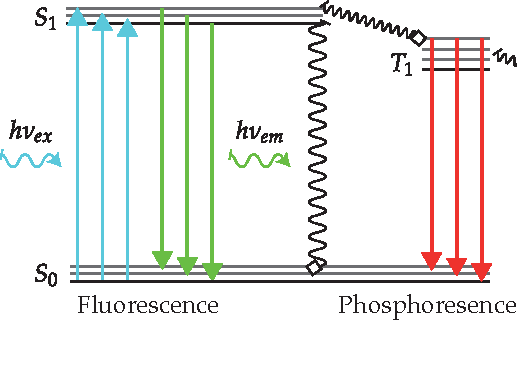
\includegraphics[width=0.7\linewidth]{jablonski_triplet}
\caption[Standard jablonski diagram]{Jablonski diagram representing in colour the excitation of Alexa Fluor\(^{\copyright}\) 488 in a standard two level fluorescent system.}\label{fig:jablonski}
\end{figure}


%\paragraph{Quantum Yield}~

%The quantum yield (\(Q_f\) of a fluorescent substance is a descriptor of how many photons are pumped in versus how many are then observed.
%For instance, the likelihood of Alexa Fluor\copyright 488 (a standard Fluorescent dye) emitting a photons when in the first excited state is 91 \%.
%A high quantum yield is a very favourable in fluorescent microscopy as it means the sample does not need to be bombarded over-zealously in an attempt to produce an observable fluorescent signal.

\subsubsection{Fluorescence Lifetime}\label{sec:lifetime}

Fluorescence lifetime is a valuable extra dimension of information exploited in biological imaging.
The time an electron spends in the excited state will vary randomly but it will be governed by a probability; the longer the electron is in this high energy state the fewer electrons in a population will also be excited.
If one were to excite a population of fluorescent molecules into an excited state the population would begin to decay with an associated time constant \(\tau\), see Equation\eqref{eq:rateeq}.
\(Q_{21}\) is a non-radiative process that has a direct environmental dependence with an impact on \(\tau\), as a result the decay constant can be affected (and therefore measure) by a multitude of factors including photochemistry, local viscosity\cite{Suhling2012}, temperature\cite{Schaerli2009}, pH and more.

\begin{align}
[S_1] (t) &= [S_1]_0 e^{-\frac{t}{\tau}}\label{eq:rateeq}\\
&\text{where}\nonumber\\
\tau = &\frac{1}{\underbrace{A_{21}}_{\text{Radiative}} + Q_{21}}
\end{align}

\subsubsection{Photo-bleaching} \label{sec:photobleaching}

%As an impulse of light causes a fluorescent decay so does a consistent exposure of light cause the decay of a population of a sample.
%his process is called photo-bleaching and occurs when a sample is illuminated so much that the photochemistry of the molecules is altered.
If a molecule for instance is excited to a singlet excited state \([S_1]\) but decays atypically to a triplet state \([T_1]\) photo-bleaching may occur, see Figure\ref{fig:jablonski}.
In the triplet state the molecule is then susceptible to covalent reaction inhibiting the typical fluorescent reaction.
 Molecules in triplet states tend to also have longer lifetimes as the decay process from a triplet state is normally forbidden in terms of radiative decay.
Explicitly for microscopy photo-bleaching is named fading as it literally means a sample that is imaged over an extended time will produce less fluorescent signal and fade.

\subsubsection{Photo-toxicity}

As well as fluorophores photo-bleaching due to exposure, biological specimens can be overly exposed to light.
Most biologicals are exposed to solar EM radiation regularly and most of those utilise it in some manner, as a result overly exposing a sample to photons can be toxic to them causing experimental complications and oddities in observed reactions or even death.
A reasonable standard to consider as a ``safe" exposure for a biological is that of the solar constant; it is a fair assumption that most biologicals are capable of surviving the Sun as they have evolved in that manner.
The Sun has a solar constant of \(\sim\SI{1}{\kilo\watt\per\meter\squared}= \SI{1}{\nano\watt\per\micro\meter\squared}\), assuming \SI{10}{} minutes of exposure is also safe that would imply an energy density of  \(\sim \SI{0.6}{\micro\joule\per\meter\squared}\).
A cell diameter is \(\sim\SI{100}{\micro\meter}\) and an embryo diameter is \(\sim \SI{900}{\micro\meter}\) meaning they should only be exposed to tens of millijoules and hundreds of millijoules respectively\cite{Stelzer2015}.

\subsection{Widefield Fluorescent  Microscopy}

%The fluorescent microscope has impacted microscopy tremendously.
The key concept behind the fluorescent microscope is the ability to separate excitation and emission.
Classical optical microscopes as well as electron microscopes both had the %very real
problem of separating these signals.
Non-fluorescent optical microscopy employed many techniques including dark field and phase contrast microscopy to avoid this problem, however they could not address it so fundamentally\cite{Murphy2012e}.
Through fluorescence the signal retrieved from the sample is chromatically labelled. %, meaning the wanted signal and the unwanted signal have different colours.
The invention of the dichroic mirror allowed these signals to be physically redirected and therefore detected completely independently.
Excitation and emission filters are used to improve light source spectra and limit scattered light emissions, see Figure\ref{fig:filtercube}.

%The notion is similar to that of the 3D glasses phase of the mid 80s.
%A projector would project both images of left and right eye superimposed to the viewing audience; a viewer without glasses saw a mixed non-3D signal, with the glasses each eye saw the correct image as the glasses filtered the unnecessary and confusing information creating a 3D effect.

%\subsubsection{Filter Cube}

%The equivalent of the 80s 3D glasses in an epi-fluorescent microscopy is dichroic filter cube.
%In signal processing unmixing two or more signals alone is a lax and poor mechanism, the unmixed signals need to be cleaned to ensure each are fully independent.
%The dichroic filter cube is at the heart of the fluorescence microscope splitting and cleaning signals.
%It uses: an excitation filter, to ensure the excitation light is of the correct colour (especially useful if the source is a broad spectral source); a dichroic mirror to redirect the emitted sample information and an emission filter to ensure that any partially reflected, unwanted light signal is fully omitted, see Figure

\begin{figure}
	\centering
	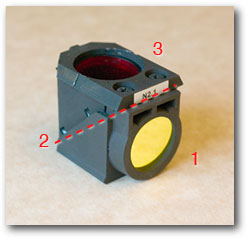
\includegraphics[width=0.3\linewidth]{filtercube}
	\caption[Fluorescent filter cube]{Standard fluorescent filter cube.
	(1) Excitation filter (2) Dichroic mirror (3) Emission barrier}
	\label{fig:filtercube}
\end{figure}
\subsubsection{Limitations}

\paragraph{The Point Spread Function}~

\textbf{Spatial resolution} is the ability of an observer to physically distinguish two close objects in an image\cite{Tsekenis2015}.
Wide-field microscopes are classically limited to \SI{250}{\nano\meter} resolution as the wavelength of visible light is of this magnitude\cite{Bradbury1998}.
Within a microscope the true limiter is the impulse response of a lens when passing light.
A lens, when focussing and magnifying, can be thought of as a low pass filter; it permits low resolution information up until a cut-off frequency.
In the Fourier plane this filtering is a circle of radius:

\begin{align}
k_r = n\frac{2 NA}{\lambda}
\end{align}

The inverse transform of this frequency filtering produces the function convolved with the sample being imaged, the \textbf{P}oint \textbf{S}pread \textbf{F}unction.
See Figure\ref{fig:Airy_Disc} for a graphical interpretation.

\paragraph{The Rayleigh Limit}~

Lord Rayleigh appraised a limit of resolution in an optical system in terms of the separation of two Airy disc point spread functions.
Rayleigh defined the limit as the distance when the maximum of the PSF is positioned on top of the first minima of the other.
This definition implies a contrast between the two functions of \SI{27}{\percent}; if the intensity trough seen from two airy discs in a microscope is lower than that, then by Rayleigh's criterion (see Equation\ref{eq:rayleigh}) the two objects cannot confidently be resolved, see Figure\ref{fig:rayleighlimit}.

\begin{figure}
	\centering
	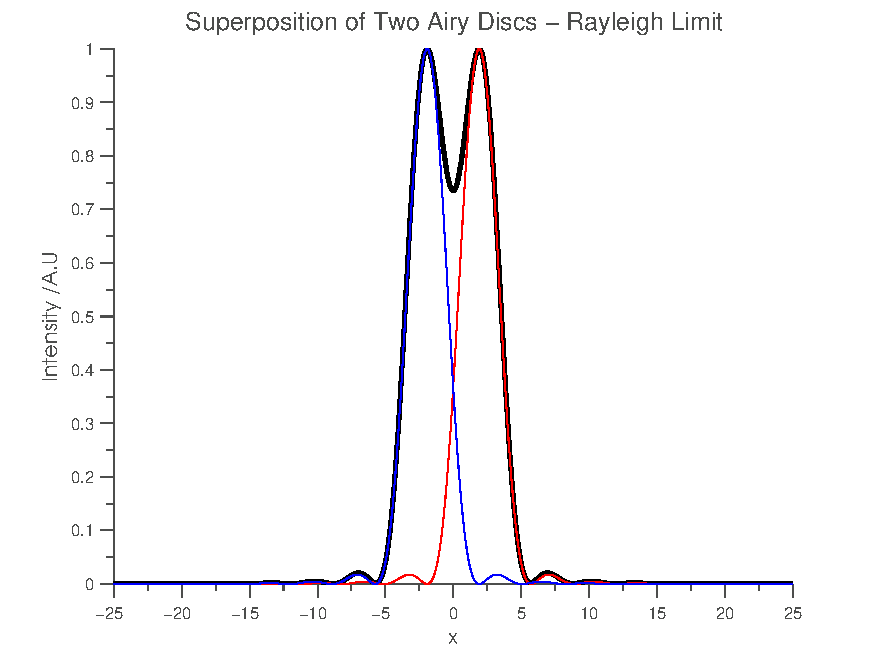
\includegraphics[width=0.7\linewidth]{rayleighlimit}
	\caption[Rayleigh Limit]{Two identical objects separated such that they are "barely resolved", the contrast (intensity difference) between their superposition being 73\% of the intensity maximum.}
	\label{fig:rayleighlimit}
\end{figure}
\begin{align}
r = \frac{\lambda}{2nNA}=\frac{1}{k_r}\label{eq:rayleigh}
\end{align}
%Optical magnification not directly improve the spatial resolution, it expands and stretches an image.
Non-optical far field techniques can resolve much smaller than the diffraction limit.
 %These techniques are limited in resolution by the size of their \textit{probe};
However, each is limited in its biological imaging capacity.
%An electron microscope would not only kill any biological sample but to properly image the sample it needs to be coated in a conductive material to ensure charge does not accumulate.
Electron microscopy uses electrons instead of photons to observe Angstrom sized particle\cite{Ruska1941}.
An electron microscope is limited by its De Broglie wavelength, the effective size of an electron, on the pico meter scale\cite{Ahmed2011,Bradbury1998}.
Electron microscopes are impractical for \textit{in vivo} biological studies, as high intensity electron beams require conductive dissipater coatings which impede and damage biological processes.

Atomic force microscopes use sensitive piezo crystals to position and record surface information from samples using a cantilever at the nanometre scale\cite{Binnig1988}.
The tip of an AFM is convolved with the profile of the surface and so is limited in resolution to the size of an atom.
Atomic force microscopes are slow raster scanning imaging techniques but more crucially offer no sample specificity, which is requisite to biology as it involves querying how two biological agents interact or how an agent acts in environment: e.g  observing diseased cell interactions in a mouse brain model\cite{Misgeld2006}, monitoring cancerous tumours\cite{Hoffman2005} and understanding virus structure\cite{Pereira2012}.

\begin{figure}
	\centering
	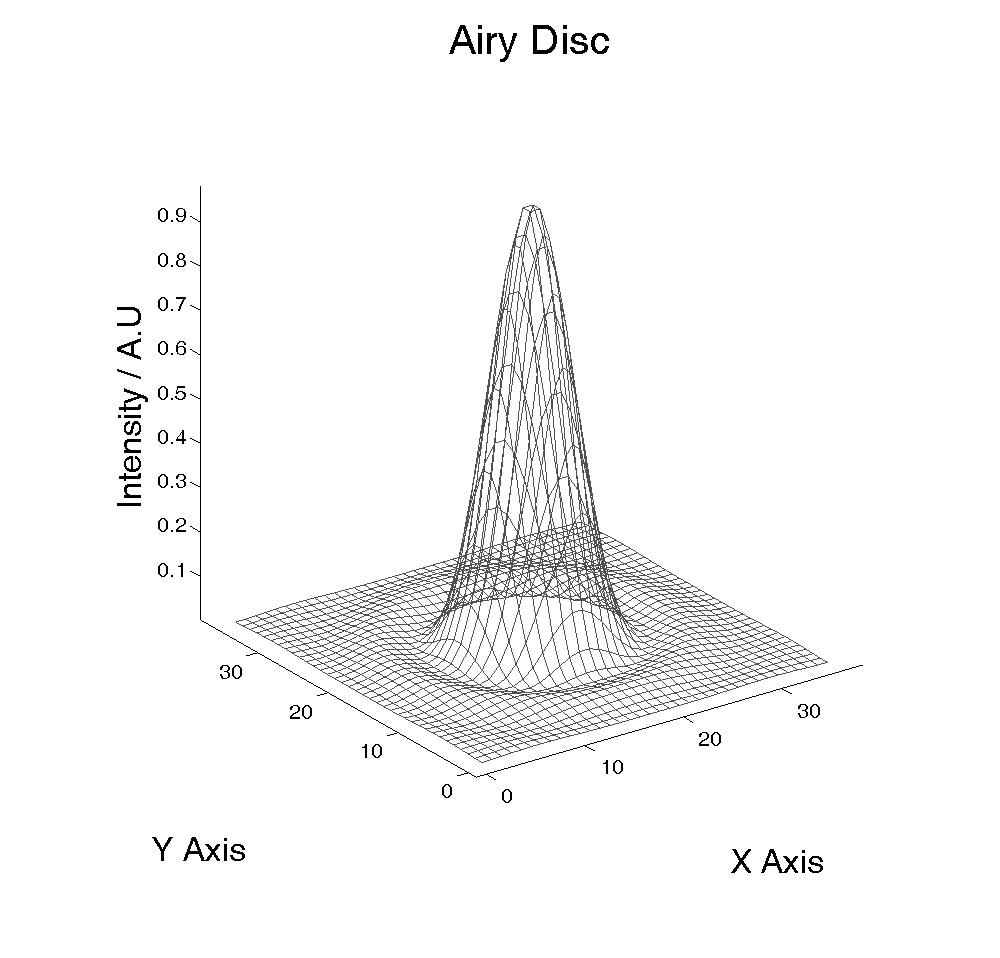
\includegraphics[width=0.6\linewidth]{Airy_Disc}
	\caption[Airy Disc]{Graphic representing the point spread function in arbitrary units of a lens.
This function is convolved with any sample being imaged through its respective lens.}
	\label{fig:Airy_Disc}
\end{figure}


%\subsection{Image Sensing}
%
%Dark Current
%Flat field
%Windowing and shutters

\section{Three Dimensional Imaging in Life Sciences}


  \begin{figure}
  \centering
  \def\svgwidth{0.6\textwidth}
  \input{Chapters/intro/Figs/PDF/guassian_waist.pdf_tex}
  \caption{You a consistent beaut \(\sqrt2 w_0\)}
  \end{figure}

%\subsection{Introduction}

Thick biological samples cannot be imaged well in classical optical microscopes.
The depth of field of the point spread function and general occlusion caused by imaging through material meant that biologists would historically mechanically section their samples in preparation.
Mechanical sectioning is highly invasive which is why Zsigmondy originally suggested (1912) the ultra-microscope as a way optically sectioning\cite{Mappes2012}.
This technique involved shining sunlight through a very narrow slit perpendicular to the optics of the microscope.
Transmitted light microscopes relied on lighting beneath the sample and the eyepiece positioned above, this technique was proposed to alleviate out of focus light blurring the image of the sample.
However, the difficulty and inherent mechanical issues of the technique meant that confocal microscopy by Marvin Minksy (1957)\cite{Minsky1957} became the standard tool of biological imaging.

\subsection{Confocal Microscopy}

Confocal microscopy offers several advantages whilst also being entirely compatible with current fluorescent labelling techniques.
By placing a small pin hole in the detector arm of a standard epi-fluorescent microscope, out of focus light from above and below the focal plane is rejected\cite{Minsky1957}, see Figure\ref{fig:confocal_optical}.
This intrinsically allows microscopy in three dimensions, in thick biological samples with an improved axial and lateral resolution improvement over wide-field\cite{Claxton2006}, see Figure\ref{fig:confocal_otf}.
Confocal microscopy does have its disadvantages too; the pin hole in the detection arm means that the image needs to be constructed by raster scanning a point of light through a sample, which is slow.
This can be achieved using a Nipkow disc or a pair of conventional galvanometer mirrors whose angle is dependent on input voltage.
The use of this pin-hole has severe consequences in terms of photon efficiency.
Firstly, the majority of the photons emitting from the sample are discarded, meaning that to get a good, high contrast image in a wide-field microscope will require a less intense light source.
Secondly, as mentioned in Section\ref{sec:photobleaching} most confocal microscopes use light intensities in the ``multiple-suns" regime\cite{Stelzer2015}, which as discussed, is likely to be an unnatural level of exposure.

%%PEDRO

Three-dimensional imaging of anatomy in thick biological samples provides valuable data for developmental biology studies.
Tomographic techniques that generate 3D reconstructions from 2D images such as computed tomography (CT) and magnetic resonance imaging (MRI) are essential in medical applications to visualize morphology in large tissues and organs.
CT and especially micro-CT can achieve micron-scale resolution using certain contrast agents, however the high doses of radiation used make this unsuitable for repeated experiments on a biological sample.
Micro-MRI can also achieve resolution in the micron scale, however the cost and size of MRI instruments can be prohibitive for many applications[21].

Furthermore, neither of these techniques can exploit the plethora of information that can be extracted through fluorescence microscopy.
Several light microscopy techniques developed in the last few decades address the shortcomings of these tomographic techniques:
High Resolution Episcopic Microscopy (HREM) [36] creates volume data sets of thick tissue samples at high resolution.
The technique is based on histological imaging, as the specimen is embedded in a fluorescent resin block and is imaged as it is being sectioned (the word episcopic comes from images taken directly from the cutting surface of the resin
block) [35].
Images are taken from the block face so they are inherently digitally aligned, and the depth resolution is determined by the number of sections. HREM requires histological sample preparation and therefore cannot be used with live samples.
%%PEDRO

\subsubsection{Two Photon Microscopy (2P)}
%Typical epi-fluorescent microscopy lacks optical sectioning due to out of focus light mixing with in focus light.
%This additional light is an effective noise which is ideally omitted.
In confocal microscopy out of focus light is removed by using a pinhole in the focal plane; the fluorescent dye in the out of focus areas of the sample will still be exposed to this out of focus light and so photo bleaching still occurs but with there is better optical sectioning\cite{Helmchen2005}.
Two photon microscopy optically sections by exploiting fluorophores which only emit when two photons are present for excitation, for this to occur the local photon density has to be high and so the focal point is the only place where fluorescent emission is likely to occur.

\begin{figure}
\centering
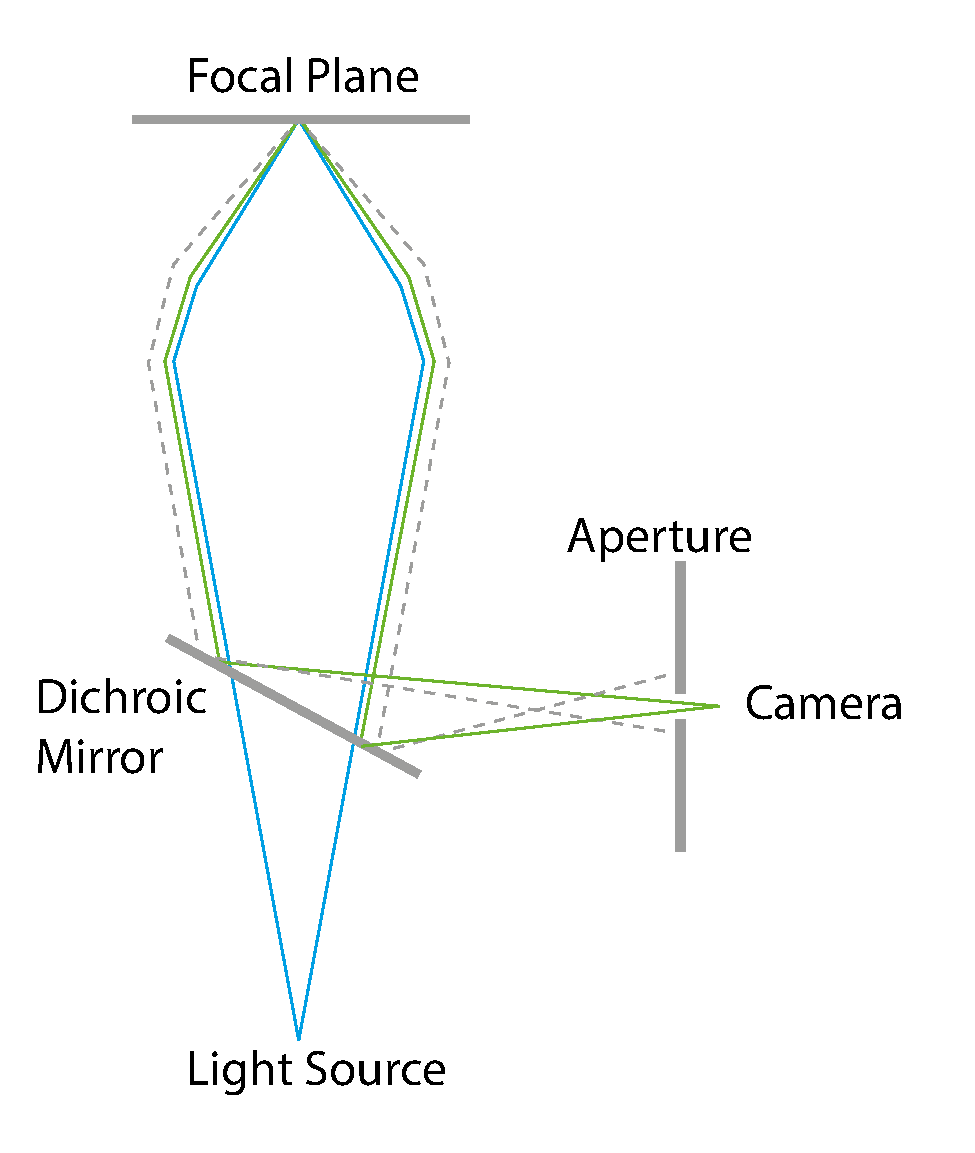
\includegraphics[width=0.4\linewidth]{confocal_optical.pdf}
\caption[Confocal microscope principle]{Confocal microscopes reject out of focus light in the detection path, improving axial and lateral resolution for the sake of speed of image acquisition and photo-toxicity.}
\label{fig:confocal_optical}
\end{figure}

\begin{figure}
	\centering
	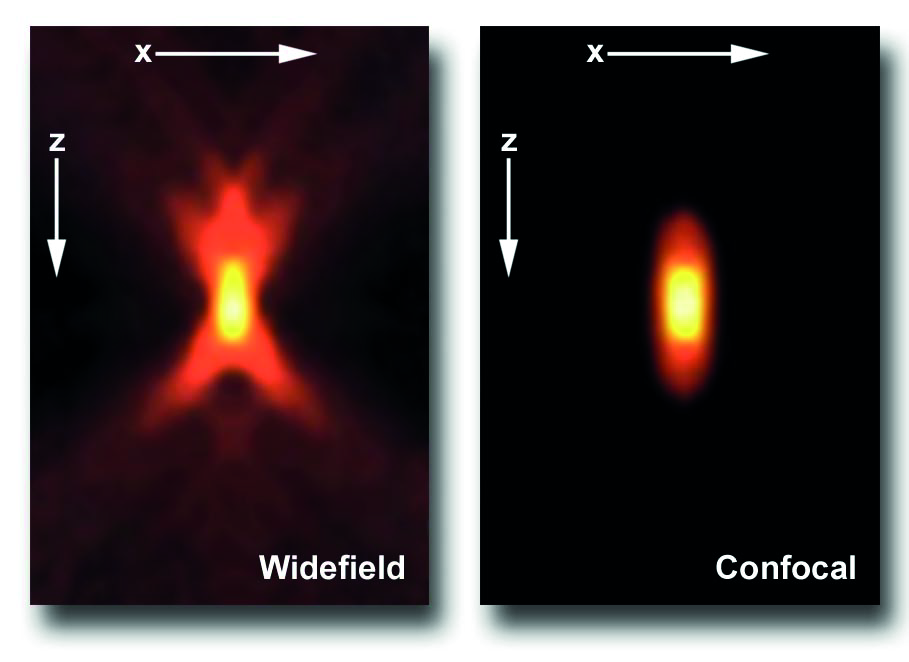
\includegraphics[width=0.7\linewidth]{confocal_otf}
	\caption[Confocal resolution improvement]{Widefield versus confocal point spread function demonstrating axial and lateral resolution improvements\cite{Claxton2006}}
	\label{fig:confocal_otf}
\end{figure}

%%PEDRO
Confocal Fluorescence Microscopy [2] enables high resolution imaging by rejecting outof- focus light from the region of interest using a pinhole in a plane conjugate to the image plane.
This technique is effective at generating volumetric data non-invasively with optical sectioning for fluorescently labelled specimens, however it is limited to thicknesses
of up to a few hundred micrometers.
Confocal microscopy works by exciting fluorescent molecules; therefore, it cannot detect signals from unlabeled tissue surrounding the fluorescent area.
Selective Plane Illumination Microscopy (SPIM) [16] can generate 3D data from biological specimens (up to a few millimeters in size) non-invasively with optical sectioning at
high resolution.
This is achieved by illuminating the sample with a thin sheet of light in the focal plane of the detection objective (generated by a cylindrical lens or by a set of scanning mirrors [19, 18],and imaging the resulting fluorescence from the excited region in an orthogonal direction.
The penetration depth of SPIM is fundamentally limited by tissue scattering, which can be partially overcome by introducing additional excitation and detection optics [32].
This increases the complexity and cost of implementation to image thick samples.

Optical Coherence Tomography (OCT) [15] allows non-invasive cross-sectional imaging of in-vivo biological samples by using low-coherence interferometry.
A fiber optic Michelson interferometer is used to illuminate the sample and collect the reflected light from tissue, which is then combined with the reflection from the reference mirror.
An 3 interference signal is only detected when the group delay of the sample and the reference arm are almost matched (close to equal time-of-flight), and this signal falls off steeply with delay mismatch due to the low-coherence nature of the light source.
This allows the longitudinal location of the reflected tissue signal to be detected with high resolution.
OCT has a limited depth of penetration due to absorbing properties of tissue, therefore it is often not suitable for whole organism imaging except in early stages of embryonic development [31].
Optical Projection Tomography was first proposed by Sharpe in 2002 [30]; it uses visible light to image and create volumetric data of transparent (naturally or artificially) mesoscopic objects (1 - 10 mm) at micron-level resolution.
OPT is based on well-documented computerized tomography techniques [17] in which a set of images (we will refer to these as projections) of an object are acquired with a camera at discrete steps over a full rotation.
A cross-sectional stack of slices from the original object is reconstructed using a back-projection algorithm from the projection images.
OPT is non-invasive (although it may require fixed samples), and it can image in two different modalities: emission OPT (eOPT) and transmission OPT (tOPT).
In eOPT, a fluorescent sample is excited using a wide-field illumination source.
The photons emitted by a fluorophore of interest are collected by a detector with an appropriate filter to reject the incident illumination.
In tOPT, a broadband source with a diffuser and a collimator lens located on the optical axis (as shown in figure 1) directs quasi-collimated, uniform illumination onto the sample.
The intensity collected at the camera is a function the amount of light absorbed by the sample.
In other words, the image recorded by the detector is a projection of the attenuated radiation that traverses the sample.
These two modalities can work together to display fluorescent signals in the context of the whole organism anatomy.
OPT attempts to address the scale gap between the tomographic techniques described above (samples larger than 10 mm), and light microscopy techniques (samples smaller than 1 mm) to image biological samples in the 1-10 mm regime.
%%PEDRO


\subsection{Selective Plane Illumination Microscopy Principles}
By using orthogonal illumination and detection (as in Figure\ref{fig:huisken_spim_setup}) \textbf{S}elective \textbf{P}lane \textbf{I}llumination \textbf{M}icroscopy is fast and less photo-toxic than confocal microscopy and two photon with only slightly lower lateral and axial resolution.
A typical diode laser in a SPIM will supply up to \SI{100}{\milli\watt} in a beam waist of \SI{3}{\micro\meter}  with an area of \SI{\sim7}{\micro\meter\squared}  which is \SI{\sim14}{\micro\watt\per\meter\squared} meaning its toxicity is in that of the ``single sun" regime.
Depending on the field of view SPIM can be as little as 500 times faster than confocal as it does not need to acquire its signal by raster scanning, point-wise.
SPIM has permitted the studies of \textit{in vivo} whole samples typically for developmental biology\cite{Huisken2004,Verveer2007a} with minimal photo-toxic repercussions.
Its advantages have been successfully demonstrated where the several day development embryos of \textit{Drosophila} \cite{Huisken2004} and Zebrafish\cite{Mickoleit2014} have been observed.

\begin{figure}
\centering
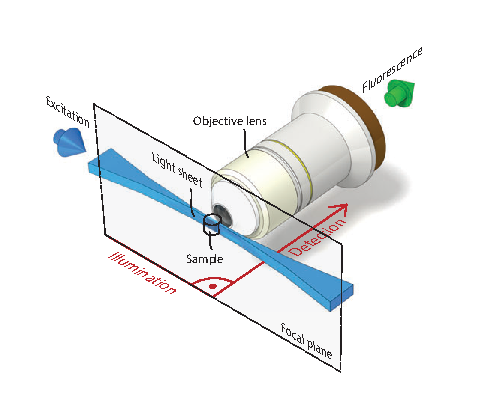
\includegraphics[width=0.7\linewidth]{huisken_spim_setup}
\caption[Single Plane Imaging Microscope principle]{Diagram demonstrating the geometrical configuration of illumination and objective\cite{Huisken2009}.}
\label{fig:huisken_spim_setup}
\end{figure}

\subsubsection{Modalities}

Orthogonal illumination can be created in two modalities.
A cylindrical lens can be used to image a light source onto a sample as a thin sheet of light.
\textbf{d}igitally \textbf{S}canned \textbf{L}ight sheet \textbf{M}icroscopy uses galvanometer mirrors to rapidly scan a thin light source through a sample\cite{Keller2008}.
Using cylindrical lenses to create a light sheet is implicitly faster than digitally scanned light sheets, however the bottleneck with each is due to the exposure time of the camera. %High frame rates produce low contrast.
A galvanometer mirror can oscillate at tens of kilohertz which is a hundred fold faster than typical sCMOS cameras can capture.
The major advantage of a cylindrical lens is that it is cheaper and more easily aligned than its counterpart the galvanometer scan mirror, which is why projects like \textit{OpenSPIM}\footnote{\textit{OpenSPIM} is a project to bring affordable light sheet microscopy to scientists who have little or no experience with optics, engineering or hardware interfacing.
Projects like this and \textit{OpenSIM} ensure that the technology is freely available to benefit everyone so that biological and medical understanding can be furthered efficiently and universally.}\cite{Gualda2013,Pitrone2013} make use of cylindrical lenses to ensure SPIM is more available and affordable to lay builders and users.
For the expense and technical ability needed for dLSM it does offer advantages such as better optical sectioning, a more homogeneous field of view and crucially the ability to positively exploit effects of the system, such as confocal slit scanning.

\subsubsection{Confocal Slit Scanning} %TODO remove

Confocal slit scanning is a technique which heavily exploits the scanning nature of dLSM.
sCMOS cameras in SPIM systems expose all the pixels equally in a frame, a shutter then rolls exporting all the pixel values so that each pixel of the current frame is synchronised and the final image is not torn or sheared.
Confocal slit scanning exposes several rows of camera pixels with roughly equal width to  the scanning laser beam.
This area of active pixels is rolled synchronously with the movement of the laser scanning.
The result is a virtual slit that confocally improves the resolution and contrast of a captured image though potentially needing more photons to create an image of the same overall intensity\cite{Baumgart2012}.

\subsubsection{Exotic illumination}

SPIM is fundamentally limited in terms of field of view and axial resolution when using classical illumination.
A typical light sheet created using a cylindrical lens or virtually will have a beam waist, a section along the propogating wave where its thickness is its smallest.
As such, light used to optically section a sample will not propagate uniformly and this thickness expands more steeply the narrower the beam waist is\cite{Silfvast2004}.
Betzig et al demonstrated very successfully how Bessel beam illumination can be exploited.
By creating an annular ring of light in the Fourier plane a narrow propagating and self reconstructing light sheet can be produced\cite{Chen2014}.
Crucially the beam waist and extension of this type of illumination profile has no dependence, so the field of view homogeneity can be maintained whilst squeezing the light sheet to a diffraction limited thickness.
Bessel beams can be created online using spatial light modulators, as well as offline using phase masks.

\paragraph{Spatial light modulators}~

A \textbf{S}patial \textbf{L}ight \textbf{M}odulator is a digitally addressable two dimensional surface which can control either phase or intensity of incident light at any of its pixels.
To this end one can create dynamic structure in illumination, which would be very difficult classically. %However, this bastion of optical manipulation is also limited.
The pixel nature of an SLM means that the reflected light will suffer from artefactual noise.
To correct for this, incident light impinges the SLM at a shallow angle (to ensure the image is not sheared, Hamamatsu recommends a maximum \(5^o\) angle)  where the exit light does not follow the optical path through the remainder of the system.
Instead this ``zero order" light is absorbed by a beam block, and the desired modified wave front is steered using a projection on the SLM.

Not any phase or intensity pattern can be projected either, each pixel will have a limited pitch with quantised steps through its dynamic range.
This means that if two neighbouring pixels need very large phase differences compared to the full dynamic range, sample issues may cause incident light to behave unpredictably.

SLMs are typically made using liquid crystals, nematic or ferroelectric.
Ferroelectric liquid crystals are very fast (\SI{\sim 500}{\hertz}\cite{Meadowlark2015}) but are limited to binary phase or intensity.
Nematic liquid crystals can rotate proportionate to electric field voltage allowing continuous phase modulation but are slow in comparison (\SI{\sim 60}{\hertz}\cite{Hamamatsu2015}).
Liquid crystals can also suffer photo damage, though advances in coating technology and liquid crystal chemistry have set the intensity damage threshold to limits outside of those used by visible light microscopy; liquid crystals however are still susceptible to light with wavelengths outside of typical operations.
Wavelengths below \SI{400}{\nano\meter} being damaging for Hamamatsu's SLMs for instance\cite{Hamamatsu2015}.

\subsubsection{Tunable Lens Scanning}\label{sec:tunable}

A tunable lens is a device which can perturb the focus of a deformable lens, usually liquid (deformed by electro-wetting) or plastic (mechanical deformation).
The change in lens curvature affects the focal length of the tunable lens.
Using a pair of tunable lenses allows sufficient degrees of freedom to be able to control both the position and extension of the light sheet independently.
Changing the focal length of the lenses so that the light is collimated but the magnification of the excitation beam at the back aperture (which controls the NA) of the objective is larger, this will extend the beam (increasing the beam waist), whilst changing the focal lengths (so that the excitation light at the back aperture is convergent or divergent) will reposition the beam waist of the light sheet further away or closer to the objective\cite{Chmielewski2015}.

This level of fine control enables one to circumvent the typical trade off between light sheet extension and thickness.
By stitching several thin light sheet images obtained at different depths in the sample, creates an overall higher resolution image for the sacrifice of speed and photo-toxicity.
Changing the position of the light sheet (when its extension is short) as it is scanned through the sample means one can \textit{bend} the light sheet around an area of interest, increasing resolution of key components of a sample and greatly reducing overall photo-toxic effects.

%TODO figure?
